\section{Introduction}
\subsection{Motivation and Background}
Since the publication of the Fortran 2008 in 2010~\cite{iso2010information}), Fortran supports a \gls{spmd} programming style
that facilitates the creation of a fixed number of replicas of a compiled program that execute asynchronously after creation.
Fortran refers to each replica as an image.  The primary mechanism for distributing and communicating data between
images involves defining \glspl{coarray}, entities that may be referenced or defined on one image by statements executing on
other images. As such, a coarray defines a \gls{pgas} and one image referencing or defining a coarray entity on another image
necessites inter-image communication of program data.

The seminal role that \glspl{coarray} played in the development of Fortran's intrinsic parallel programming model have made it
common to refer to all of modern Fortran's parallel programming features under the rubric of \gls{caf}.  To date, most
published disucssions \gls{caf} in applications involve scenarios wherein the parallelization itself poses one of the chief
challenges and necessitates the custom development of parallel algorithms.  These include ordinary and partial differential
equation solvers in domains ranging from nuclear fusion~\cite{preissl2011multithreaded} and
weather~\cite{mozdzynski2015partitioned} to multidimensional fast Fourier transforms and multigrid numerical
methods~\cite{garain2015comparing}.  Much of the effort involved in expressing parallel algorithms for these domains centers
 using \gls{caf} centers around designing and using various \gls{coarray} data structures.  In such settings, the moniker
\gls{caf} seems appropriate.

Less widely appreciated are the ways in which Fortran's intrinsic parallel programming model supports embarassingly parallel
applications: problems in which the division into sub-problems that execute in parallel with little or no coordination between
the sub-problems.  To support such applicaitons, a parallel programming model might provide for the explicit disaggregation
and independent execution of sub-problems in ways that do not require the user to declare, reference, or define \glspl{coarray}.
The upcoming Fortran 2015 standard (expected to be published in 2018\footnote{A Committee Draft is at
https://bit.ly/fortran-2015-draft.}) will provide several features that enable a considerable amount of parallel computation
without the use of \glspl{coarray}.  These include the ability to declare teams of images that communicate only with each
other by default.

In the context of \gls{caf}, we propose a working definition of ``embarassingly parallel'' as denoting the class of parallel
applications that can be addressed without the need for \glspl{coarray}.  In addition to the ability to form teams, Fortran
2015 supports this application class with mechanisms for ordering program segments in differing images; collective subroutines
containing highly optimized implementations of common parallel communication and computation patterns; and global error
termination.  We anticipate that a common teams use case for these capabilities will involve running an ensemble of simulations,
each member of which executes in a separate team.  This paper presents such a use case in the context of a terrestrial
hydrological model developed at \gls{ncar}: the \gls{wrf-hydro}.

For the work described herein, we wrote what we believe to be the first compiler and runtime-library implementations of Fortran
2015 teams.  In addition to providing an open-source platform for studying the application of teams, our implementation offers a
language extension that assists with incrementally introducing \gls{caf} into existing \gls{mpi} applications.
Section~\ref{sec:objectives} of this paper details the objectives for using teams in \gls{wrf-hydro}.
Section~\ref{sec:methodology} provides an overview of teams in Fortran 2015, the open-source \gls{gcc} fork we established to
supports teams, and the \gls{wrf-hydro} teams use case.

\subsection{Objectives}\label{sec:objectives}
For both validation purposes and production use, multiple instances of \gls{wrf-hydro} often run on a parametric family of
input data.  Although each point in the phase space of interest represents an independent simulation, much of the problem
initiationalion remains invariant across the parameter space.  One therefore expects to achieve considerable reductions in
execution time by amortizing the initialization across all available computational resources rather than repeating common
aspects of the initialzation in each ensemble member using only that member's fraction of the hardware resources available to
each. Section~\ref{sec:discussion} pre

\section{Methodology}
\subsection{Teams in Fortran 2015}\label{teams-in-fortran-2015}
The existing coarray definition in Fortran 2008 does not provide for an environment
where a subset of the images can easily work on part of an application without affecting
other images in the program.  Grouping the images of a program into nonoverlapping
teams allows one to execute more effectively and independently parts of a larger
problem.  A class of problems that can benefit from this feature is multiphysics codes
(e.g.  climate models).
Such feature, called \textit{Teams} in the Fortran 2015 standard, can significantly reduce the amount of off-node
communication on an exascale machine, in particular when an entire team of images
fits within a single compute node.
So far, the only compiler with a partial support for this new feature is the GNU Fortran Compiler (from now on
called GFortran) and a special version of the OpenCoarrays library.
In this Section we are going to introduce the basic constructs of \textit{Teams} and how OpenCoarrays implements them.

A team of images is a set of images that can readily execute independently of other images.
Initially, the current team consists of all images and this is
known as the initial team. Except for the initial team, every team has a unique parent team. A team is divided
into new teams by executing a \texttt{FORM TEAM} statement.
Each new team is identified by an integer value known
as its team number. Information about the team to which the current image belongs can be determined by the
processor from the collective value of the team variables on the images of the team.
The \texttt{FORM TEAM} statement is a collective operation executed by all the images.

During execution, each image has a current team, which is only changed by execution of \texttt{CHANGE TEAM} and
\texttt{END TEAM} statements. Executing a \texttt{CHANGE TEAM} statement changes the current team to the team specified
by the team-variable, and execution of the corresponding \texttt{END TEAM} statement restores the current team back
to that immediately prior to execution of the \texttt{CHANGE TEAM} statement.

Teams are described by a scalar variable called \texttt{TEAM TYPE}. This variable is a derived type with private components.
The \texttt{FORM TEAM} statement takes as first argument a team number that uniquely identifies the team and a \texttt{TEAM TYPE}
variable as second argument.
Successful execution of a \texttt{FORM TEAM} statement assigns the team-variable (of type \texttt{TEAM TYPE}) on each
participating image a value that specifies the new team that the image will belong to.
The \texttt{CHANGE TEAM} statement takes as argument a \texttt{TEAM TYPE} variable that represents the new team to be used as
current team. The execution of the \texttt{END TEAM} statement restores the current team back
to that immediately prior to execution of the \texttt{CHANGE TEAM} statement.

\subsection{Teams in \gls{gcc} and OpenCoarrays}\label{subsec:teams-in-gcc}

From an MPI prospective, a Fortran team is comparable to an MPI communicator. The \texttt{FORM TEAM} statement is implemented in OpenCoarrays
using \texttt{MPI\_Comm\_split} and passing the team id argument as \textit{color} for \texttt{MPI\_Comm\_split}.
In case of success, the resulting communicator is stored into a list of available teams.
Every element of the list keeps track of the association of team id and actual MPI communicator.
The elements of the list of available teams gets returned by the function and stored into the \texttt{TEAM TYPE} variable.

When the \texttt{CHANGE TEAM} statement gets invoked, the element of the list of available teams stored into the \texttt{TEAM TYPE} variable
gets passed as argument to the correspondent OpenCoarrays function. The \texttt{current\_team} variable used inside OpenCoarrays for
representing the current communicator gets reassigned with the value contained into the element of the list passed as argument.
Finally, a new element is added to the list of used teams. This list of element is nothing but a list of pointers to the elements of the list
of available teams. The insert operation is always performed at the beginning of the list in order to keep track of the teams hierarchy.

An execution of the \texttt{END TEAM} statements is implemented by removing the first element of the list of used teams and reassigning the
\texttt{current team} to the new first element of the list of used teams.

The list of available and used teams are both initialized to team 1 (equivalent to \texttt{MPI\_COMM\_WORLD}) at the beginning of the execution.

\begin{figure*}
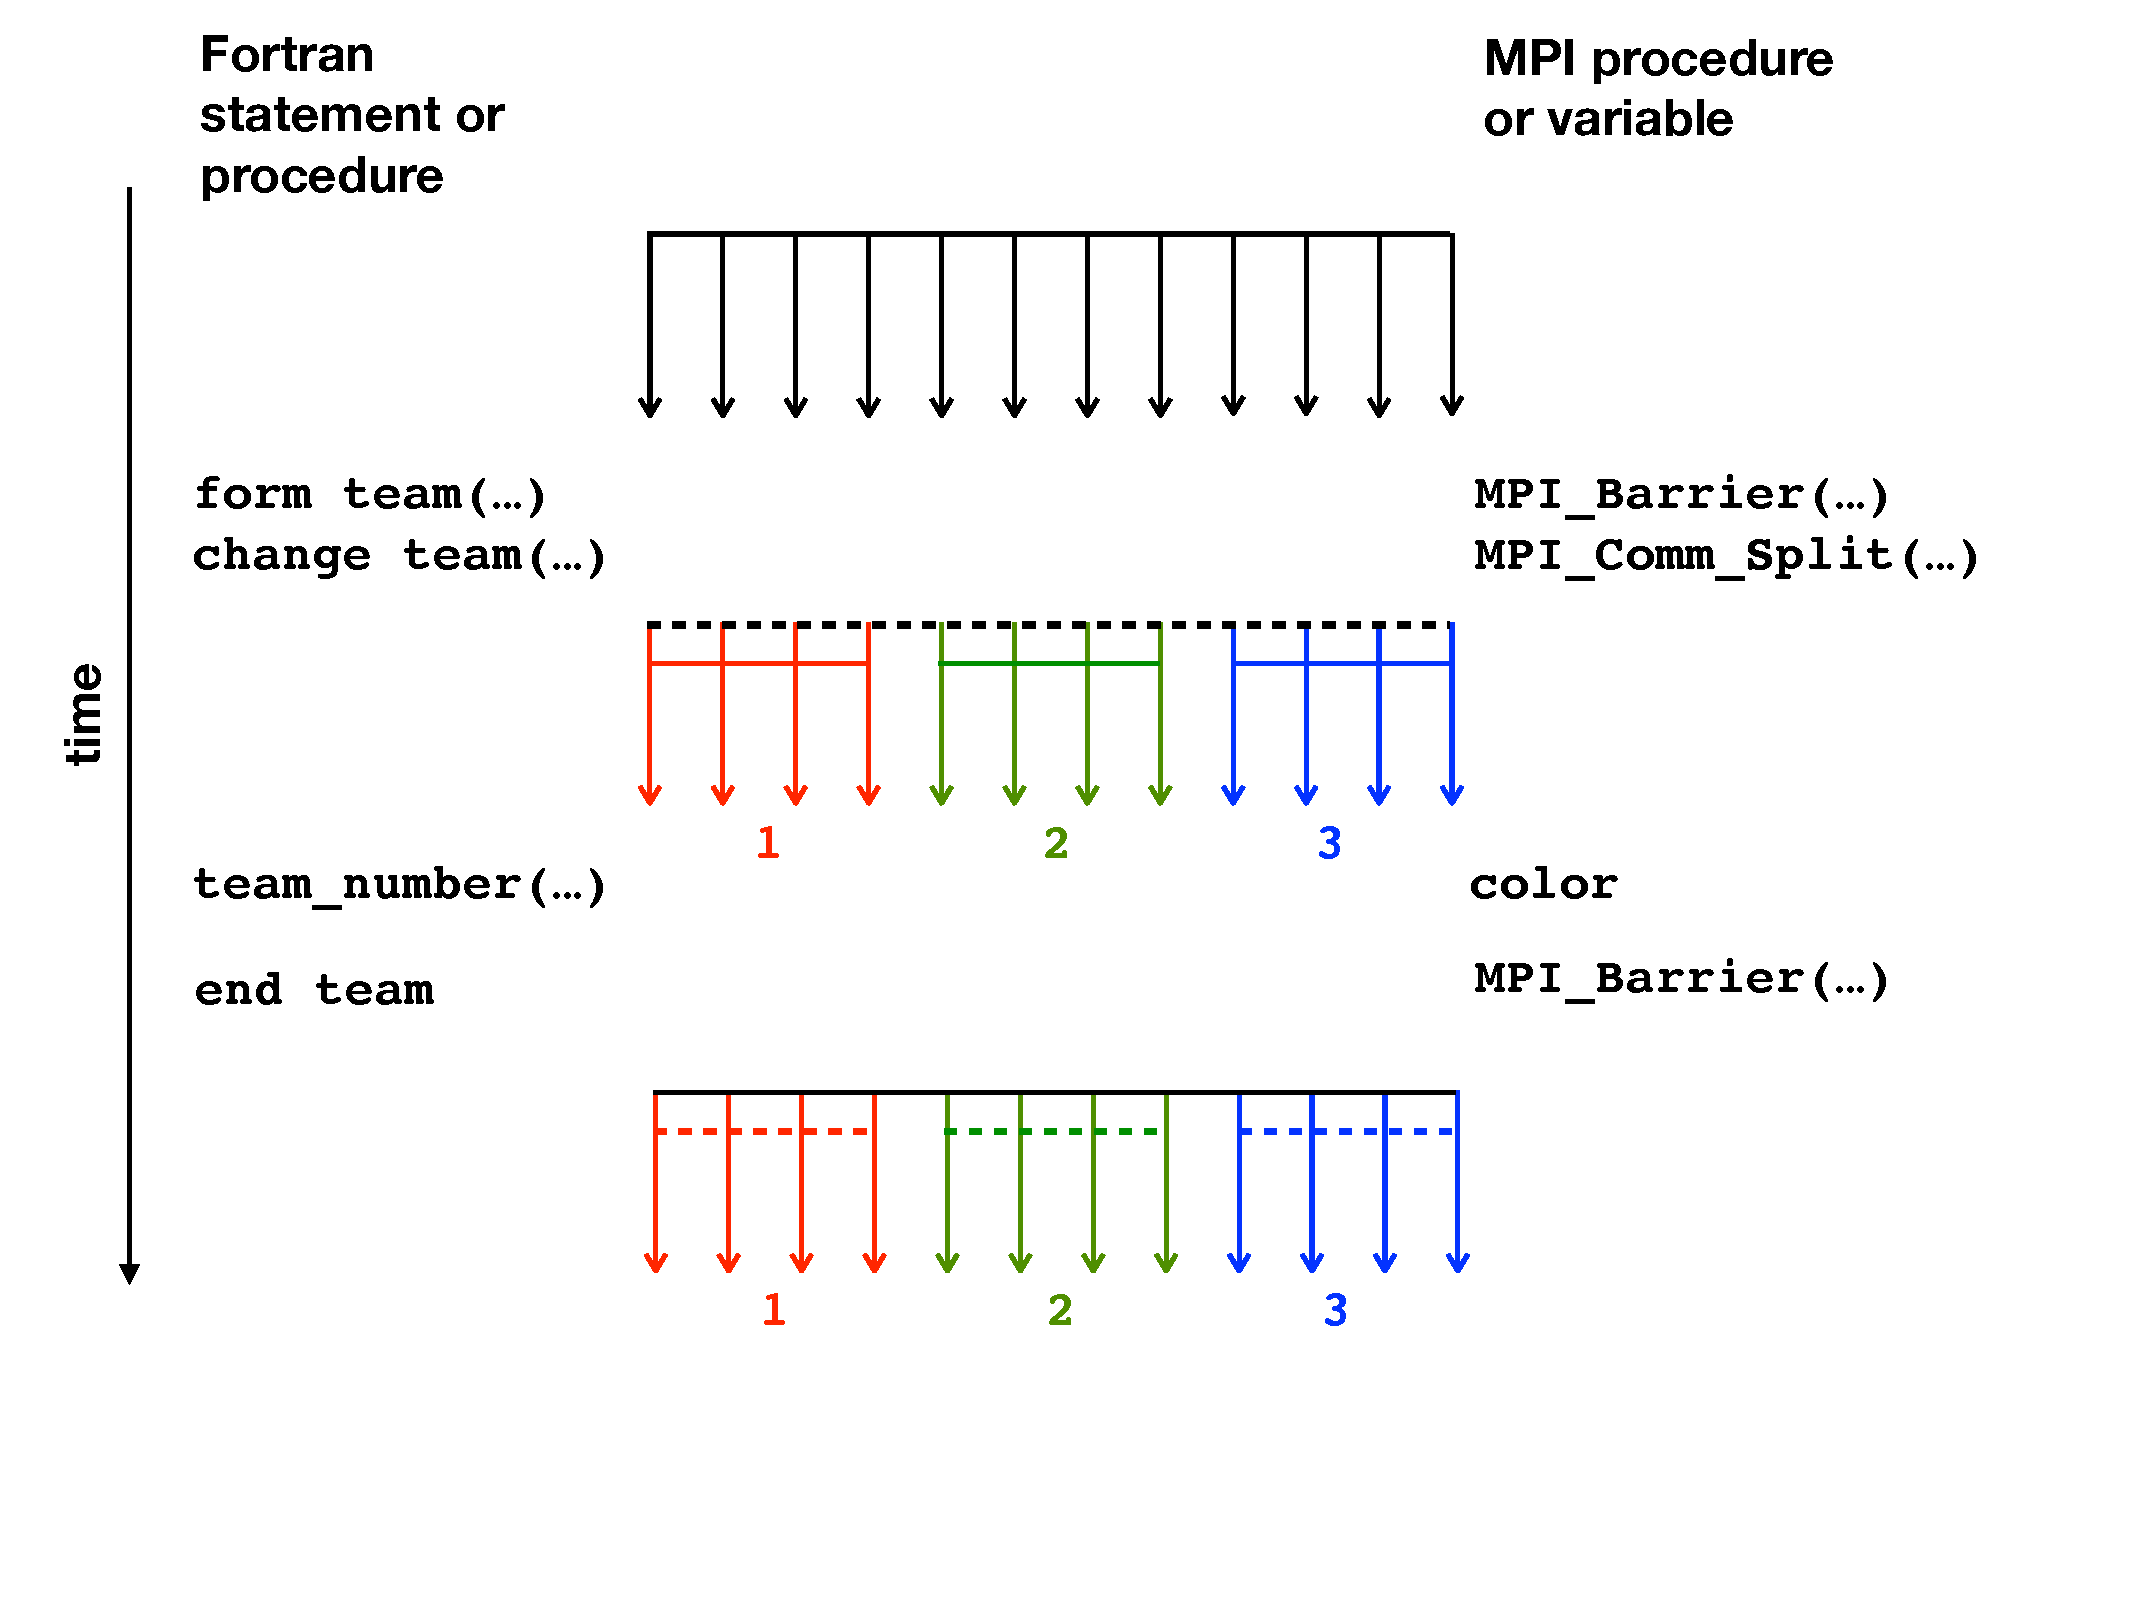
\includegraphics[width=0.7\textwidth]{figures/teams}
\vspace{-36pt}
\caption{Schematic depiction of a Fortran program executing over time (left axis) in 12 images (top) thatcommunicate with each other through global means (black horizontal bar) and later communicating within subgroups (colored horizontal bars).  Horizontal lines represent the communication mechanisms (default=solid, optional=dashed).  Fortran concepts or on the left.  The underlying \gls{mpi} concepts are the right.}
\end{figure*}
%

\begin{figure*}
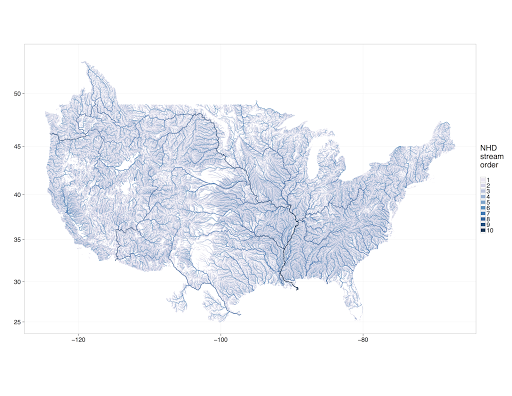
\includegraphics[width=0.7\textwidth]{figures/hydro-map}
\vspace{-36pt}
\caption{Sample \gls{wrf-hydro} simulation domain.}
\end{figure*}
%

\subsection{Teams in \gls{wrf-hydro}}
\section{Discussion of Results}
\section{Conclusions}

%%%
%%% Sample tables
%%%

%\begin{table}
%  \caption{Frequency of Special Characters}
%  \label{tab:freq}
%  \begin{tabular}{ccl}
%    \toprule
%    Non-English or Math&Frequency&Comments\\
%    \midrule
%    \O & 1 in 1,000& For Swedish names\\
%    $\pi$ & 1 in 5& Common in math\\
%    \$ & 4 in 5 & Used in business\\
%    $\Psi^2_1$ & 1 in 40,000& Unexplained usage\\
%  \bottomrule
%\end{tabular}
%\end{table}

%\begin{table*}
%  \caption{Some Typical Commands}
%  \label{tab:commands}
%  \begin{tabular}{ccl}
%    \toprule
%    Command &A Number & Comments\\
%    \midrule
%    \texttt{{\char'134}author} & 100& Author \\
%    \texttt{{\char'134}table}& 300 & For tables\\
%    \texttt{{\char'134}table*}& 400& For wider tables\\
%    \bottomrule
%  \end{tabular}
%\end{table*}
% end the environment with {table*}, NOTE not {table}!

%It is strongly recommended to use the package booktabs~\cite{Fear05}
%and follow its main principles of typography with respect to tables:
%\begin{enumerate}
%\item Never, ever use vertical rules.
%\item Never use double rules.
%\end{enumerate}
%It is also a good idea not to overuse horizontal rules.


%%%
%%% Sample figures
%%%

%\begin{figure}
%\includegraphics{fly}
%\caption{A sample black and white graphic.}
%\end{figure}

%\begin{figure}
%\includegraphics[height=1in, width=1in]{fly}
%\caption{A sample black and white graphic
%that has been resized with the \texttt{includegraphics} command.}
%\end{figure}

%\begin{figure*}
%\includegraphics{flies}
%\caption{A sample black and white graphic
%that needs to span two columns of text.}
%\end{figure*}
%
%\begin{figure}
%\includegraphics[height=1in, width=1in]{rosette}
%\caption{A sample black and white graphic that has
%been resized with the \texttt{includegraphics} command.}
%\end{figure}

%\end{document}  % This is where a 'short' article might terminate



\appendix
%Appendix A
\section{Teams unit tests}
% This next section command marks the start of
% Appendix B, and does not continue the present hierarchy

\begin{figure*}
  \lstinputlisting{figures/tests/get-team.f90}
  \caption{A unit test for the get-team function.\label{figure:get-team-test}}
\end{figure*}

%\begin{figure*}
%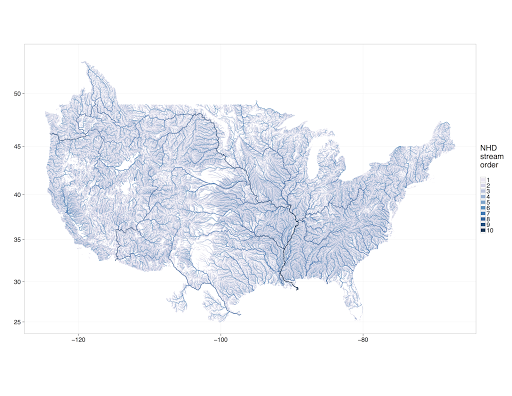
\includegraphics[width=0.7\textwidth]{figures/hydro-map}
%\vspace{-36pt}
%\caption{Sample \gls{wrf-hydro} simulation domain.}
%\end{figure*}
%

\begin{figure*}
  \lstinputlisting{figures/tests/team-number.f90}
  \caption{A unit test for the team-number function.\label{figure:team-number-test}}
\end{figure*}


\begin{acks}
  The authors would like to thank the CISL and RAL Visitor Program

  The work is
  supported by the \grantsponsor{GSxxxxx}{National
  Science Foundation China}{http://dx.doi.org/zz.yyyyy/xxxxx} under Grant
  No.:~\grantnum{GSxxxxx}{yyyyyyy}

\end{acks}
